%%%%%%%%%%%%%%%%%%%%%%%%%%%%%%%%%%%%%%%%%%%%%%%%%%%%%%%%%%%%%%%%%%%%%%%%%%%%%%%% INIZIO %%%%%%%%%%%%%%%%%%%%%%%%%%%%
Scopo dell'esperienza è la misura dell'impedenza e della funzione di trasferimento ai capi di una capacità. Come verrà dimostrato nella sezione \ref{sec:C3_P2-1}, l'impedenza per una capacità è:  $Z_c = \frac{1}{\omega C} \; e^{-j\pi/2}$
\\
%
%%%%%%%%%%%%%%%%%%%%%%%%%%%%%%%%%%%%%%%%%%%%%%%%%%%%%%%%%%%%%%%%%%%%%%%%%%%%%%%% FDT %%%%%%%%%%%%%%%%%%%%%%%%%%%%%%%
%
\subsubsection{Funzione di trasferimento per C}
La funzione di trasferimento ai capi del componente C, $V_{b-a}/V_a$, è:
$$ H(\omega) = \frac{ V_{b-a} }{V_a} = \frac{Z_CI}{Z_{tot}I} = \frac{\frac{1}{j\omega C}}{R + \frac{1}{j\omega C}} = \frac{1}{1+j\omega CR} $$
%
per cui, modulo e argomento sono:
%
$$ Mod(H) = \frac{1}{\sqrt{ 1+(\omega R_{tot} C)^2} } \quad e \quad Arg(H) = \arctan(-\omega R_{tot}C) $$
%
Con $R_{tot} =  R + r_{gen} = 14900 \pm 200 \Omega $.
\begin{figure}[H]
    \centering
    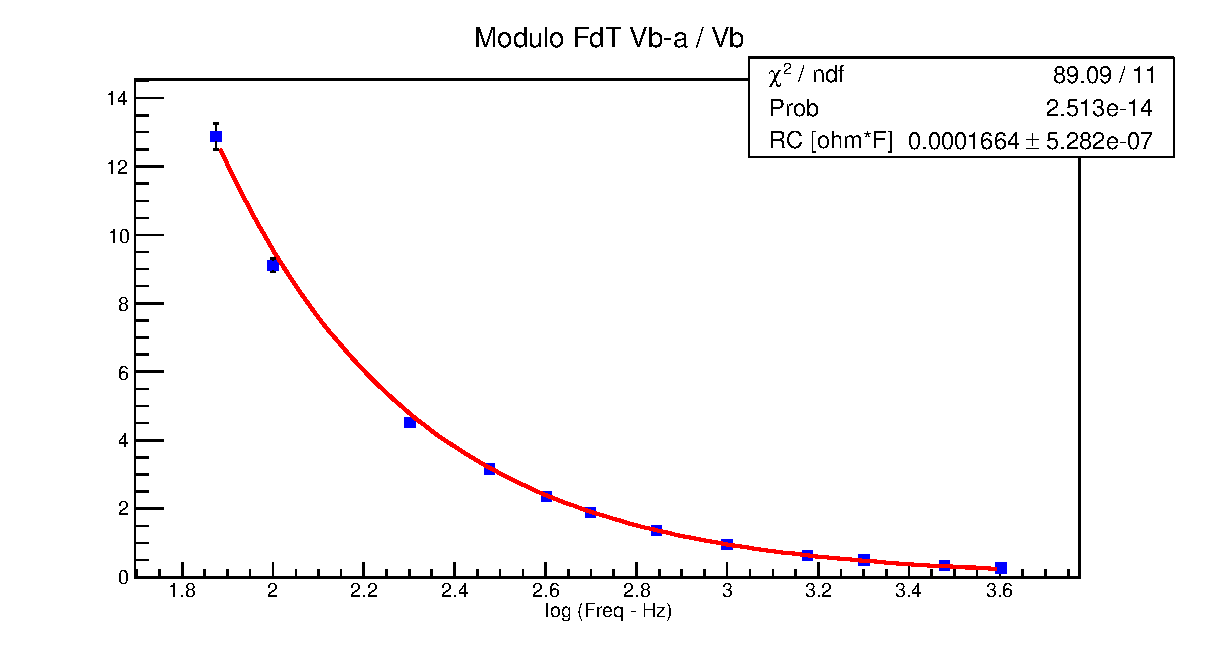
\includegraphics[scale=.6]{Grafici/C2_P2_ModFdt1_.eps}
    \caption{
        Modulo funzione di trasferimento $ \tfrac{Vba}{Vb} $.
         Capacità valore nominale $11$ $nF$
    }
    \label{fig:C2_P2_ModFdt1}
\end{figure}
%
\begin{figure}[H]
    \centering
    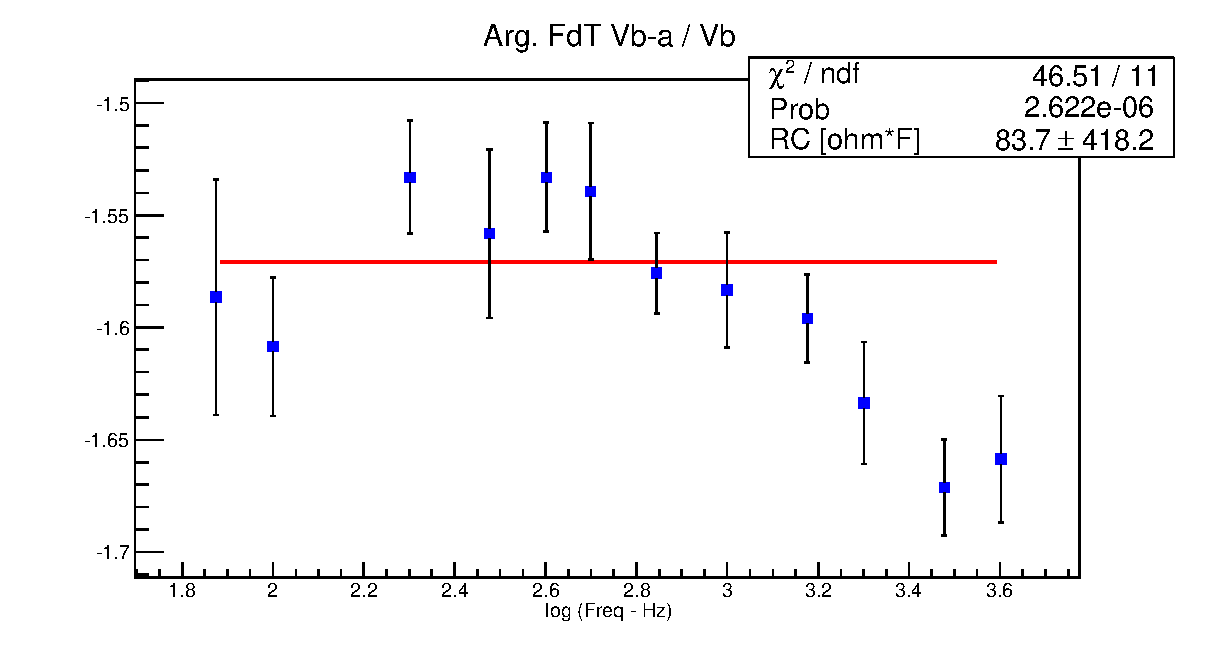
\includegraphics[scale=.6]{Grafici/C2_P2_ArgFdt1_.eps}
    \caption
    {
        Argomento funzione di trasferimento $ \tfrac{Vba}{Vb} $.
        Capacità valore nominale $11$ $nF$
    }
    \label{fig:C2_P2_ArgFdt1}
\end{figure}
%%%%%%%%%%%%%%%%%%%%%%%%%%%%%%%%%%%%%%%%%%%%%%%%%%%%%%%%%%%%%%%%%%%%%%%%%%%%%%%% IMPEDENZA %%%%%%%%%%%%%%%%%%%%%%%%%
\subsubsection{Impedenza per C}
L'impedenza per C vale $Z_C = \tfrac{1}{j\omega C}$ di modulo $ Mod(Z) = \tfrac{1}{\omega C}$ e fase $Arg(Z)= \arctan(- 1/ \omega C)$
%	C: 26200 +/- 193 nF
\begin{figure}[H]
    \centering
    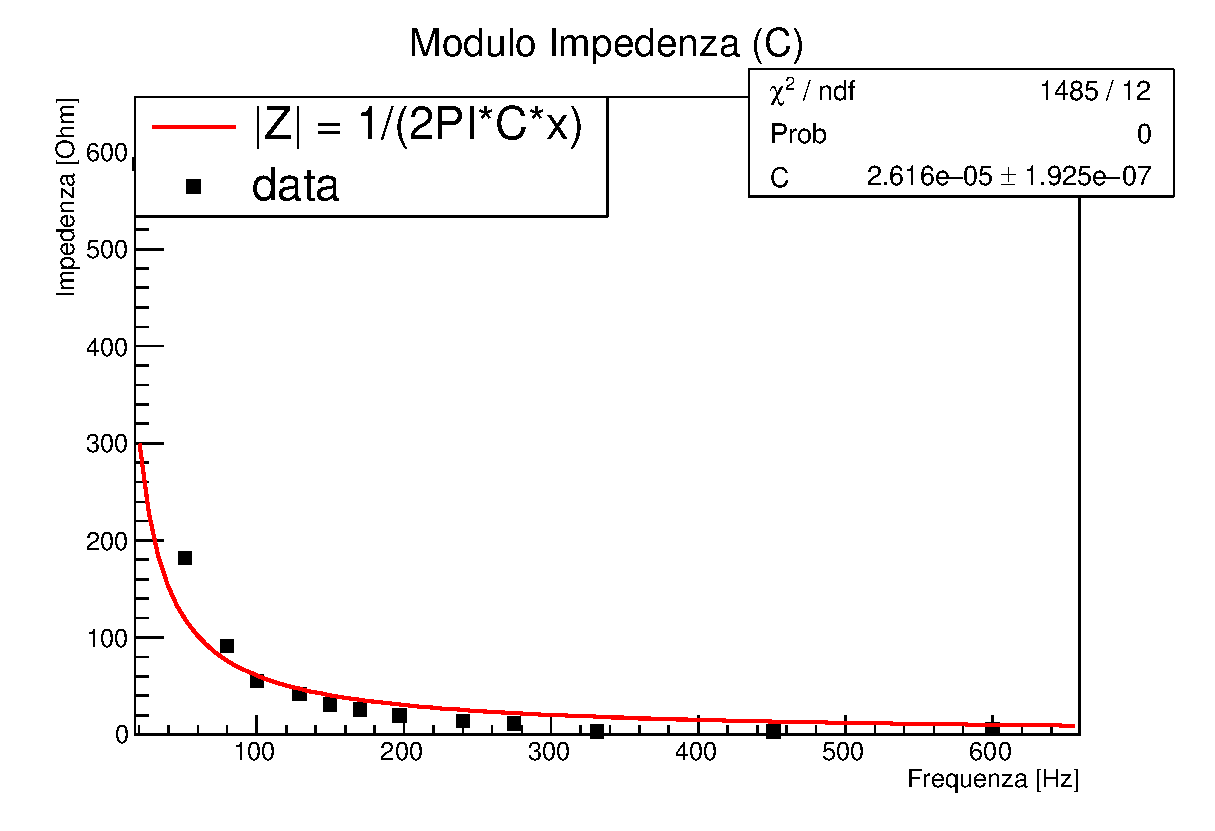
\includegraphics[scale=.7]{Grafici/C2_P2_impedenzaC.eps}
    \caption{Modulo dell'impedenza per C}
    \end{figure}

\begin{figure}[H]
    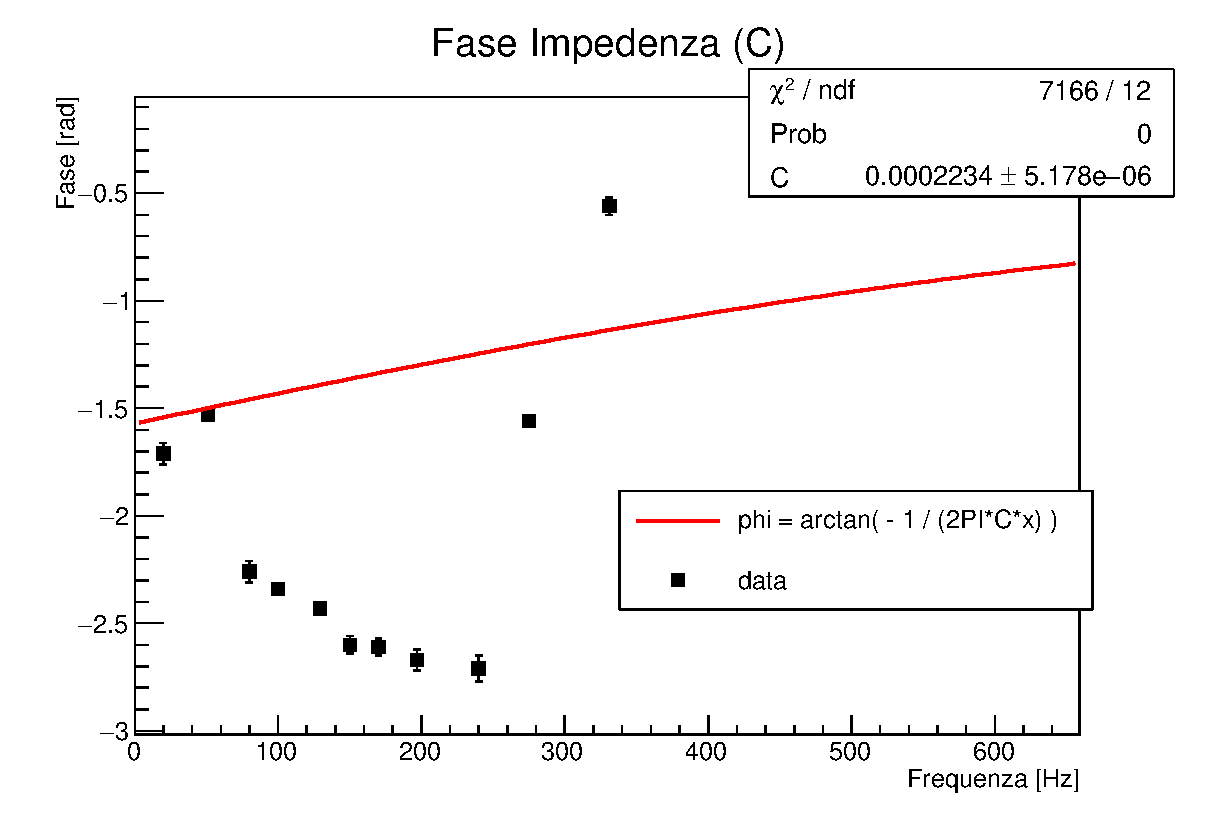
\includegraphics[scale=.7]{Grafici/C2_P2_impedenzaFaseC.eps}
    \caption{Fase dell'impedenza per C}
\end{figure}
\paragraph{Considerazioni}{I risultati dei fit producono valori di C non attendibili, considerando i $\chi^2$ ottenuti.}
%%%%%%%%%%%%%%%%%%%%%%%%%%%%%%%%%%%%%%%%%%%%%%%%%%%%%%%%%%%%%%%%%%%%%%%%%%%%%%%%
\subsubsection{Funzione di trasferimento $V_b/V_a$}
La funzione di trasferimento ai capi della resistenza R è:
  $$ H(\omega) = \frac{V_b}{V_a} = \frac{Z_RI}{Z_{tot}I} =  \frac{R \frac{V_a}{R+Z_C}}{V_a} =
  \frac{R}{R + \frac{1}{j\omega C} } = \frac{1}{j\omega CR + 1} $$
e quindi:
  $$ Mod(H) = \frac{\omega C R}{\sqrt{1 + (\omega CR)^2}} \quad \mathrm{e} \quad Arg(H) = \arctan(\frac{1}{\omega CR})$$
%
\begin{figure}[H]
    \centering
    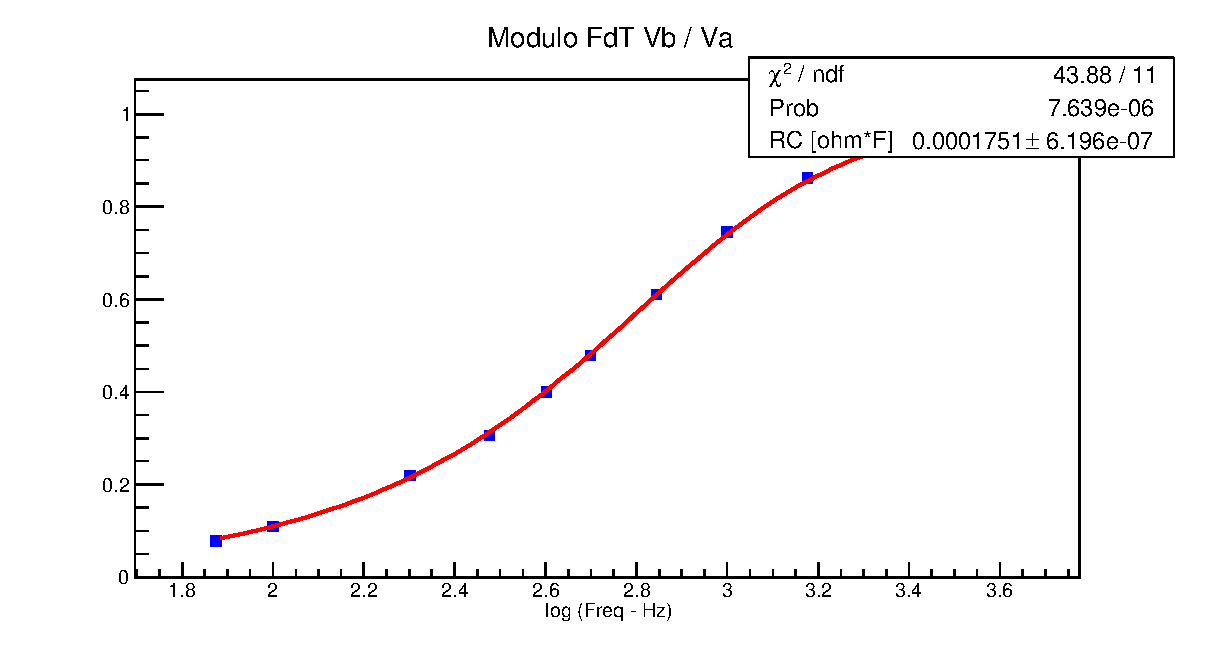
\includegraphics[scale=.6]{Grafici/C2_P2_ModFdt2_.eps}
    \caption
    {
        Modulo funzione di trasferimento $ \tfrac{Vb}{Va} $.
    }
    \label{fig:C2_P2_ModFdt2}
\end{figure}
%
\begin{figure}[H]
    \centering
    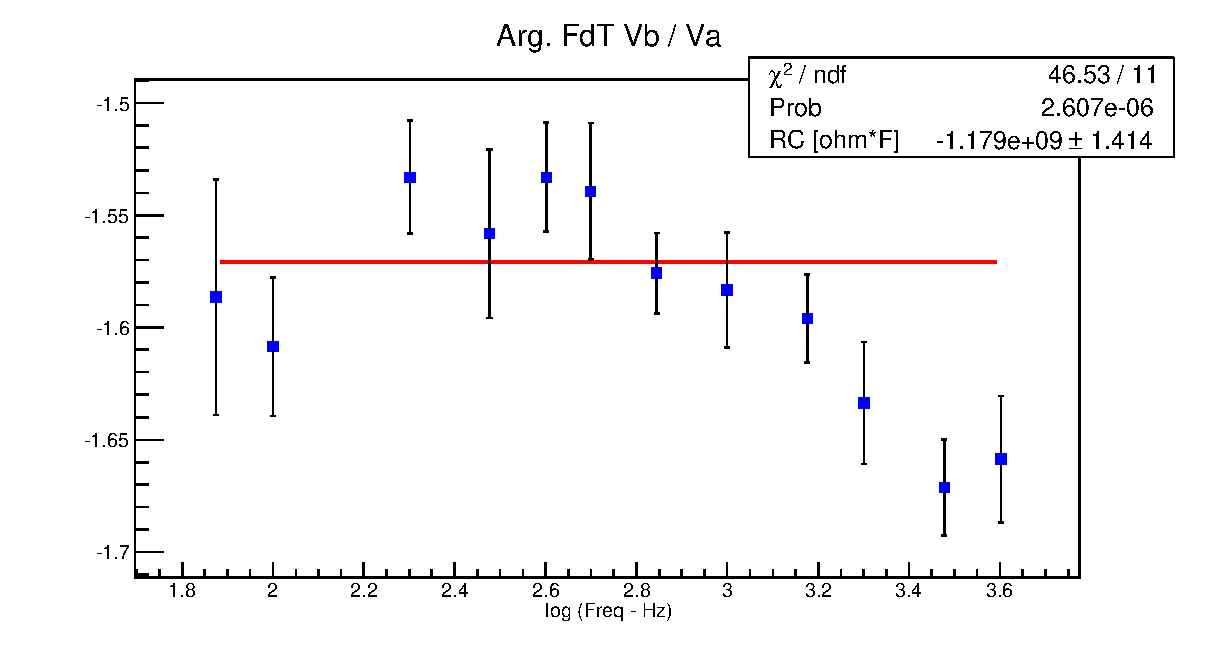
\includegraphics[scale=.6]{Grafici/C2_P2_ArgFdt2_.eps}
    \caption
    {
        Argomento funzione di trasferimento $ \tfrac{Vb}{Va} $.
        Resistenza totale $ R + r_{gen} = 14870 + 50 \pm 150 \Omega $.
        Capacità valore nominale $11$ $nF$.
    }
    \label{fig:C2_P2_ArgFdt2}
\end{figure}
%%%%%%%%%%%%%%%%%%%%%%%%%%%%%%%%%%%%%%%%%%%%%%%%%%%%%%%%%%%%%%%%%%%%%%%%%%%%%%%%%% DATI %%%%%%%%%%%%%%%%%%%%%%%%%%%%
\subsubsection{Dati}
\begin{table}[H]
\begin{center}
\begin{tabular}{|c|c|c|c|c|}
\hline
\multicolumn{ 2}{|c|}{Fdt} & $R_{tot}C$ & $C$ & $\chi^{2}$ \\ \hline
\multicolumn{ 2}{|c|}{   } & $\omega\cdot nF$ & $nF$ &  \\ \hline

\multicolumn{ 1}{|c|}{$Vba/Vb$} & mod 
& $166400\pm500$  & $11.15\pm1.3\%$ & 89/11  \\

\multicolumn{ 1}{|c|}{} & arg & - & -  &  \\ \hline

\multicolumn{ 1}{|c|}{$Vb/Va$} & mod 
& $175100\pm619$ & $11.73\pm1.3\%$ & 44 / 11  \\

\multicolumn{ 1}{|c|}{} & arg & - & - &  \\ \hline

\end{tabular}
\end{center}
\caption{
Riepilogo risultati fit.
Resistenza totale $ R + r_{gen} = 14870 + 50\pm 150$ $\Omega$.
}
\label{C2_P2_risultati}
\end{table}

\begin{table}[H]
\begin{center}
\begin{tabular}{|r|r|r|r|r|r|r|r|}
\hline
\multicolumn{1}{|l|}{Freq} & \multicolumn{1}{l|}{Va} & \multicolumn{1}{l|}{Vb} & \multicolumn{1}{l|}{Vb-a} & \multicolumn{1}{l|}{-Fase (CH2)} & \multicolumn{1}{l|}{err-(CH2)} & \multicolumn{1}{l|}{-Fase (CH1)} & \multicolumn{1}{l|}{err-(CH1)} \\ \hline
\multicolumn{1}{|l|}{Hz} & \multicolumn{1}{l|}{V} & \multicolumn{1}{l|}{V} & \multicolumn{1}{l|}{V} & \multicolumn{1}{l|}{$\mu$s} & \multicolumn{1}{l|}{$\mu$s} & \multicolumn{1}{l|}{$\mu$s} & \multicolumn{1}{l|}{$\mu$s} \\ \hline
\multicolumn{1}{|c|}{$\pm$ 1} & \multicolumn{1}{c|}{$\pm$ 0.08} & \multicolumn{1}{c|}{$\pm$ 0.08} & \multicolumn{1}{c|}{$\pm$ 0.16} & \multicolumn{1}{l|}{} & \multicolumn{1}{c|}{$\pm$ } & \multicolumn{1}{l|}{} & \multicolumn{1}{c|}{$\pm$ } \\ \hline
75 & 10.2 & 0.80 & 10.3 & 3300 & 200 & 6400 & 200 \\ \hline
100 & 10.2 & 1.12 & 10.2 & 2,440 & 80 & 4800 & 80 \\ \hline
200 & 10.2 & 2.24 & 10.1 & 1,280 & 40 & 2340 & 40 \\ \hline
300 & 10.2 & 3.12 & 9.84 & 840 & 40 & 1500 & 40 \\ \hline
400 & 10.2 & 4.08 & 9.60 & 640 & 20 & 1090 & 20 \\ \hline
500 & 10.2 & 4.88 & 9.20 & 510 & 20 & 850 & 20 \\ \hline
700 & 10.1 & 6.16 & 8.40 & 356 & 8 & 560 & 8 \\ \hline
1000 & 10.3 & 7.68 & 7.36 & 248 & 8 & 372 & 8 \\ \hline
1500 & 10.3 & 8.88 & 5.68 & 164 & 4 & 220 & 4 \\ \hline
2000 & 10.2 & 9.36 & 4.64 & 120 & 4 & 158 & 4 \\ \hline
3000 & 10.2 & 9.92 & 3.36 & 78 & 2 & 96 & 2 \\ \hline
4000 & 10.2 & 10.0 & 2.64 & 59 & 2 & 68 & 2 \\ \hline
\end{tabular}
\end{center}
\caption{
Dati relativi alle figure
\ref{fig:C2_P2_ModFdt1}
\ref{fig:C2_P2_ArgFdt1}
\ref{fig:C2_P2_ModFdt2}
\ref{fig:C2_P2_ArgFdt2}.
Condensatore valore nominale $11$ $nF$.
Resistore $14870\pm 150$ $ohm$.
}
\label{C2_P2_cond1}
\end{table}


